\documentclass[sigconf]{acmart}

%\settopmatter{printacmref=false} % Removes citation information below abstract
%\renewcommand\footnotetextcopyrightpermission[1]{} % removes footnote with conference information in first column
\pagestyle{empty} % removes running headers

\usepackage{booktabs} % For formal tables
\usepackage{multirow}
\newcommand\Tstrut{\rule{0pt}{2.6ex}}         % = `top' strut
\newcommand\Bstrut{\rule[-0.9ex]{0pt}{0pt}}   % = `bottom' strut

\usepackage{makecell}
\usepackage{hyperref}

\usepackage{amsfonts}
\usepackage{amsmath}
\usepackage{pgfplots} % for plot bar chart 
\newcommand{\floor}[1]{\lfloor #1 \rfloor}
\newcommand{\norm}[1]{\left\lVert #1 \right\rVert}

\usepackage{bm}

% Chèn và định dạng mã nguồn
\usepackage{listings}
\usepackage{color}
\definecolor{codegreen}{rgb}{0,0.6,0}
\definecolor{codegray}{rgb}{0.5,0.5,0.5}
\definecolor{codepurple}{rgb}{0.58,0,0.82}
\definecolor{backcolour}{rgb}{0.95,0.95,0.92}

% Tikz
\usepackage{tikz}
\usetikzlibrary{matrix}
\usetikzlibrary{patterns}
\usetikzlibrary{shapes.geometric, arrows}
\tikzstyle{process} = [rectangle, minimum width=1cm, minimum height=1cm, text centered, draw=black ]
\tikzstyle{io} = [rectangle, minimum width=0.5cm, minimum height=0.1cm, text centered, draw=white]
\tikzstyle{up} = [yshift=0.2cm]
\tikzstyle{arrow} = [thick,->]
\tikzstyle{sq} = [rectangle, minimum width=0.7cm, minimum height=0.7cm, text centered, draw=black ]
\tikzstyle{cir} = [circle, minimum width=0.7cm, minimum height=0.7cm, text centered, draw=black ]
\tikzstyle{sqvec} = [matrix,draw=black,thick] 
\tikzstyle{cirsmall} = [circle, minimum width=0.3cm, minimum height=0.3cm, draw=black ]
\tikzstyle{sqvec2} = [matrix,draw=black,thick] 
\tikzset{
	sq1/.style={rectangle, minimum width=1cm, minimum height=1cm, text centered, draw=black},
	sq1m/.style={rectangle, minimum width=0.8cm, minimum height=0.4cm, text centered, draw=black},
	sq1p/.style={rectangle, minimum width=1cm, minimum height=1cm, text centered, draw=black, pattern=north west lines},
	circ/.style={circle, minimum width=0.4cm, minimum height=0.4cm, text centered, draw=black},
	arrow/.style={thick,->},
	sqvec/.style={matrix,matrix of nodes,nodes in empty cells},
}

\lstdefinestyle{mystyle}{
	backgroundcolor=\color{backcolour},   
	commentstyle=\color{codegreen},
	keywordstyle=\color{magenta},
	numberstyle=\tiny\color{codegray},
	stringstyle=\color{codepurple},
	basicstyle=\footnotesize,
	breakatwhitespace=false,         
	breaklines=true,                 
	captionpos=b,                    
	keepspaces=true,                 
	numbers=left,                    
	numbersep=5pt,                  
	showspaces=false,                
	showstringspaces=false,
	showtabs=false,                  
	tabsize=2
}
\lstset{style=mystyle}

% Copyright
\setcopyright{none}
\setcopyright{acmcopyright}
\setcopyright{acmlicensed}
\setcopyright{rightsretained}
\setcopyright{usgov}
\setcopyright{usgovmixed}
\setcopyright{cagov}
\setcopyright{cagovmixed}


% DOI
\acmDOI{10.475/123_4}

% ISBN
\acmISBN{123-4567-24-567/08/06}

%Conference
\acmConference[WOODSTOCK'97]{ACM Woodstock conference}{July 1997}{El
  Paso, Texas USA} 
\acmYear{1997}
\copyrightyear{2016}

\acmPrice{15.00}


\begin{document}
\title{Combining Convolution and Recursive~Neural~Networks for Sentiment~Analysis}

\author{Vinh D. Van}
\orcid{1234-5678-9012}
\affiliation{%
	\institution{Faculty of Information Technology
		VNUHCM - University of Sciences }
	\streetaddress{Nguyen Van Cu}
	\city{Ho Chi Minh} 
	\country{Vietnam}}
\email{vdvinh@apcs.vn}

\author{Thien Thai}
\affiliation{%
	\institution{Faculty of Information Technology
		VNUHCM - University of Sciences }
	\streetaddress{Nguyen Van Cu}
	\city{Ho Chi Minh} 
	\country{Vietnam}}
\email{tthien@apcs.vn}

\author{Quoc-Minh Nghiem}
\affiliation{%
  \institution{Faculty of Information Technology
  VNUHCM - University of Sciences }
  \streetaddress{Nguyen Van Cu}
  \city{Ho Chi Minh} 
  \country{Vietnam}}
\email{nqminh@fit.hcmus.edu.vn}

% The default list of authors is too long for headers}
\renewcommand{\shortauthors}{V. Van et al.}


\begin{abstract}
This paper addresses the problem of sentence-level sentiment analysis.
In recent years, Convolution and Recursive Neural Networks have been proven to be effective network architects for sentence-level sentiment analysis.
Nevertheless, each of them has their own potential drawbacks.
For alleviating their weaknesses, we combined Convolution and Recursive Neural Networks into a new network architect.
In addition, we employed transfer learning from a large document-level labeled sentiment dataset to improve the word embedding in our models.
The resulting models outperform all recent Convolution and Recursive Neural Networks.
Beyond that, our models are able to achieve  comparable performance with the state-of-the-art systems of Stanford Sentiment Treebank.
\end{abstract}

%
% The code below should be generated by the tool at
% http://dl.acm.org/ccs.cfm
% Please copy and paste the code instead of the example below. 
%
\begin{CCSXML}
	<ccs2012>
	<concept>
	<concept_id>10002951.10003317.10003347.10003353</concept_id>
	<concept_desc>Information systems~Sentiment analysis</concept_desc>
	<concept_significance>500</concept_significance>
	</concept>
	<concept>
	<concept_id>10010147.10010257.10010258.10010262.10010277</concept_id>
	<concept_desc>Computing methodologies~Transfer learning</concept_desc>
	<concept_significance>300</concept_significance>
	</concept>
	</ccs2012>
\end{CCSXML}

\ccsdesc[500]{Information systems~Sentiment analysis}
\ccsdesc[300]{Computing methodologies~Transfer learning}


\keywords{Sentence-level Sentiment Analysis, Convolution Neural Network, Recursive Neural Network, Transfer Learning}

\maketitle

\section{Introduction}
In a nutshell, sentiment analysis is to determine whether the opinion about a specific product, event, organization is positive or negative. It is also known as opinion mining due to the sentiment was derived from opinions of the speaker.

Formally, given document $d$, The main objective of sentiment analysis is define as quintuples~\cite{liu2012sentiment}:
\[ ( e_{i}, a_{ij}, s_{ijkl}, h_{k}, t_{l} ) \]
Where:
\begin{itemize}
	\item $e_{i}$: entity i (entity extraction and categorization)
	\item $a_{ij}$: aspect j of entity i (entity extraction and categorization)
	\item $h_{k}$: holder k (opinion holder extraction and categorization)
	\item $t_{l}$: time l (time extraction and standardization)
	\item $s_{ijkl}$: opinion of holder k about aspect j of entity i at time l (aspect sentiment classification)
\end{itemize}
Sentence-level sentiment analysis is to determine whether a sentence expressed positive or negative. 
A sentence is assumed only contain opinion toward one entity (a single movie) ~\cite{liu2012sentiment}.

Before a customer buys any product, the decision of whether or not he will buy it depends largely on his prior opinions about that product.
These opinions, in turn, have been built based on his opinions on relating companies or products and other customers' opinions about that product.
After having been experiencing the product, his posterior opinions on the product not only tell us about which features he likes or not.
His opinion also informs the retailer about the reasons why he bought the product, his expectations, needs and even more his personal information.
In a circle, his opinions will also affect the opinion of new customers and even the design of future products.
As a result, customers' opinions are the controllers behind every companies' good decisions.
They shape companies' marketing strategies, policies, and designs of products.
They judge which company is more competent than another.

A long time ago, when companies needed to know opinions of their customers, they conducted surveys, opinion polls and focus groups~\cite{liu2012sentiment}.
In recent years, thanks to the dramatic growth of social media, customers' opinions are expressed in the highest speed and volume ever recorded in history.
With this amount of data, it is inefficient to read and analyze or even collect them manually. Sentiment analysis offers a way to collect and process public opinion automatically.

In search of new improvements on the task of sentence-level sentiment analysis, we have tried three approaches: Utilizing local syntactic information at each node of Recursive Neural Networks; Transfer Learning by retraining Glove on Amazon Reviews dataset and Combining Recursive Neural Networks with Convolution Neural Networks.
\textbf{Hypotheses that supported by our experiment results including}:
\begin{itemize}
	\item For sentence-level sentiment analysis on movie reviews, there exist useful features in Glove Amazon which does not exist or hardly be extracted in Glove Common Crawl.
	On the other hand, there also exist useful features that does not appear in Glove Amazon but only appear in Glove Common Crawl or when combining both Glove Amazon and Glove Common Crawl.
	
	\item By adding a convolution layer before the leaf-module of Tree-LSTM, the convolution layer will help Tree-LSTM to mitigate the problem of lacking local context and weak feature capturing at leaf nodes.
	Mutually, using Tree-LSTM to combine the feature maps produced by convolution layer is better than max-over-time pooling layer.
	
	\item  Tree-LSTMs have already utilized the information in word embeddings and the local syntactic information from tag embeddings adding no more value. 
\end{itemize}

\section{Background}
\subsection{Word Embeddings}
Mikolov et al. introduced word2vec which has the ability to learn a certain level of syntactic and semantic relationships among words~\cite{word2vec}.
Pre-learned word presentations have been used widely and become the “secret sauce” for the success of recent NLP systems~\cite{Luong_betterword}.
\paragraph{Matrix presentation of sequences of words}
Given any sentence \(s\) of length \(n\), we denote \(x_i \in \mathbb{R}^d\) as a vector presentation of word-\(i\)th in the sentence.
Note that the first word in a sentence is word-\(0\)th, if the sentence is padded with dummy words on its left, these padded dummy words are indexed by negative integers.
Any sequence of words in the sentence which start at word-\(i\)th and end at word-\(j\)th can be presented as the following:
\begin{align}
X_{i:j} &= x_i \oplus x_{i+1} \oplus ... \oplus x_{j} &\label{concat}
\end{align}
In Eq.\eqref{concat}, \(\oplus\) is concatenation operator which result in the matrix \(X_{i:j} \in \mathbb{R}^{d \times (j-i+1)}\).
\subsection{Convolution and Pooling}
Convolution Neural Networks (CNNs) have been proven to be effective models for the task of sentence-level sentiment analysis~\cite{KimCNN}.
Although being a simple Convolution Neural Network architect on top of pre-trained word embedding channels, CNN-multichannel~\cite{KimCNN} was able to archive state-of-the-art performance\footnote{2014} on Stanford Sentiment Treebank with binary setting.
Despite its success, for dealing with the problem composing fixed size presentation vectors given variable-length input sentences, CNN-multichannel utilized max-over-time pooling layer~\cite{nlp-scratch}.
\subsection{Recurrent Neural Network}
By definition, Recurrent Neural Networks are any Neural Networks which have at least a recurrent connection~\cite{rnn-def}.
\subsubsection{Vanilla Recurrent unit}\label{sec:vanilla-rnn}
Denoting input sequence as \(I = \{i_0,\ldots,i_n\}, \forall t, i_t \in \mathbb{R}^n\), Vanilla Recurrent unit can be expressed as the following recursive formula~\cite{treeLSTM}:
\begin{align}
h_t &= tanh(Wi_t + Uh_{t-1} + b)&\label{eq:rnn}
\end{align}
In Eq.\ref{eq:rnn}, \(h_t\) is called state of the system~\cite{deeplearning-book}, but we can also treat \(h_t\) as an output of the unit.

In theory, Vanilla Recurrent Neural Network is Turing-Complete~\cite{rnn-turing-complete} but  hard to train (especially on long input sequence) due to the problems of exploding and vanishing gradient~\cite{Bengio1994}.
In layman's terms, the longer the dependencies between an output and an input the (exponentially ) harder it is for the training process to capture those dependencies.
To mitigate the problem of vanishing gradient, Long Short Term Memory unit (LSTM)~\cite{originLSTM} unit was invented.
\subsubsection{Long Short Term Memory unit}\label{sec:lstm}
Given a input sequence \(I = (i_0,\ldots,i_n), \forall t, i_t \in \mathbb{R}^n\), Long Short Term Memory unit can be expressed as the following recursive formula~\cite{treeLSTM}:
\begin{align}
w_t &= \sigma(W^{(w)}i_t + U^{(w)}h_{t-1} + b^{(w)}) \label{eq:lstm-input-gate}&\\
f_t &= \sigma(W^{(f)}i_t + U^{(f)}h_{t-1} + b^{(f)}) \label{eq:lstm-forget-gate}&\\
o_t &= \sigma(W^{(o)}i_t + U^{(o)}h_{t-1} + b^{(o)}) \label{eq:lstm-output-gate}&\\
u_t &= tanh(W^{(u)}i_t + U^{(u)}h_{t-1} + b^{(u)}) \label{eq:lstm-update-gate}&\\
c_t &= r_t \otimes u_t + f_t \otimes c_{t-1} \label{eq:longterm-mem}&\\
h_t &= o_t \otimes tanh(c_t) \label{eq:temperal-mem}&
\end{align}
In the formula above, operator \(\otimes\) is the Hadamard product~\cite{element-prod}.
The role of \(h_t\) in LSTM unit is similar to its role in Vanilla Recurrent unit.
Traditionally, \(w_t\), \(f_t\) and \(o_t\) are called input/write gate, forget/deallocate gate and output/read gate respectively.
In addition, \(c_t\) is called memory cell.

Consistently, LSTM outperform Vanilla RNN in most tasks.
Intuitively, LSTM mitigates the problem of vanishing gradient by updating their memory through adding~\cite{evaluate-GRU}, although gradients still decrease through time, it is not exponentially~\cite{Graves-thesis}.
\subsection{Recursive Neural Network}
In most cases, to understand a sentence, we have to understand the phrases composing it.
Analogously, to understand a phrase, we have to understand the phrases and words composing it.
Recursive Neural Networks were mainly inspired by this idea~\cite{treeLSTM}.
Given a sentence and its parse tree, a Recursive Neural Network composes the vector presentation of the sentence by applying it composition function at each node of the parse tree in a bottom-up manner.
For demonstration, parse tree of the phrase ``is very interesting'' and its composing process using a Recursive Neural Network are illustrated in Fig.\ref{fig:example-parse} and Fig.\ref{fig:example-compose} respectively~\cite{tag-embedding-rnn}.


\begin{figure}[H]
	\centering
	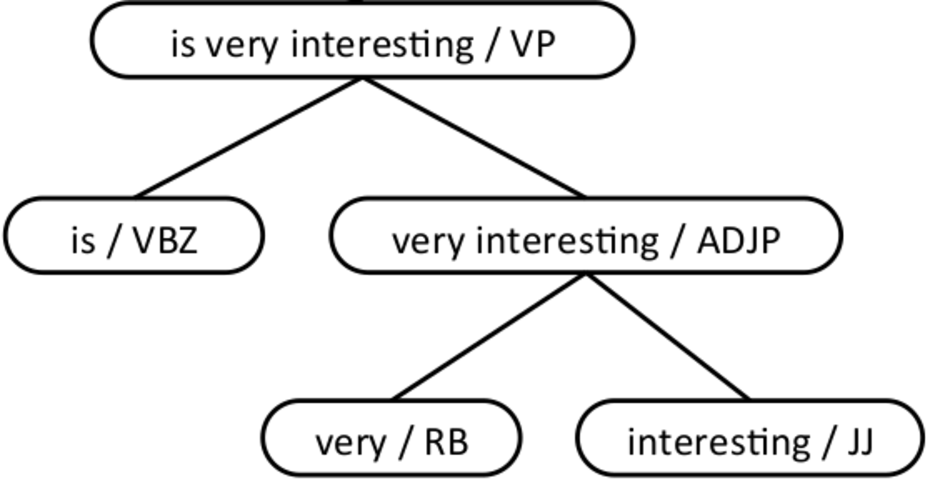
\includegraphics[scale=0.4]{figure/example-parse}
	\caption[Constituency parse tree for the phrase ``is very interesting'']{Constituency parse tree for the phrase ``is very interesting''.}
	\label{fig:example-parse}
\end{figure}

\begin{figure}[H]
	\centering
	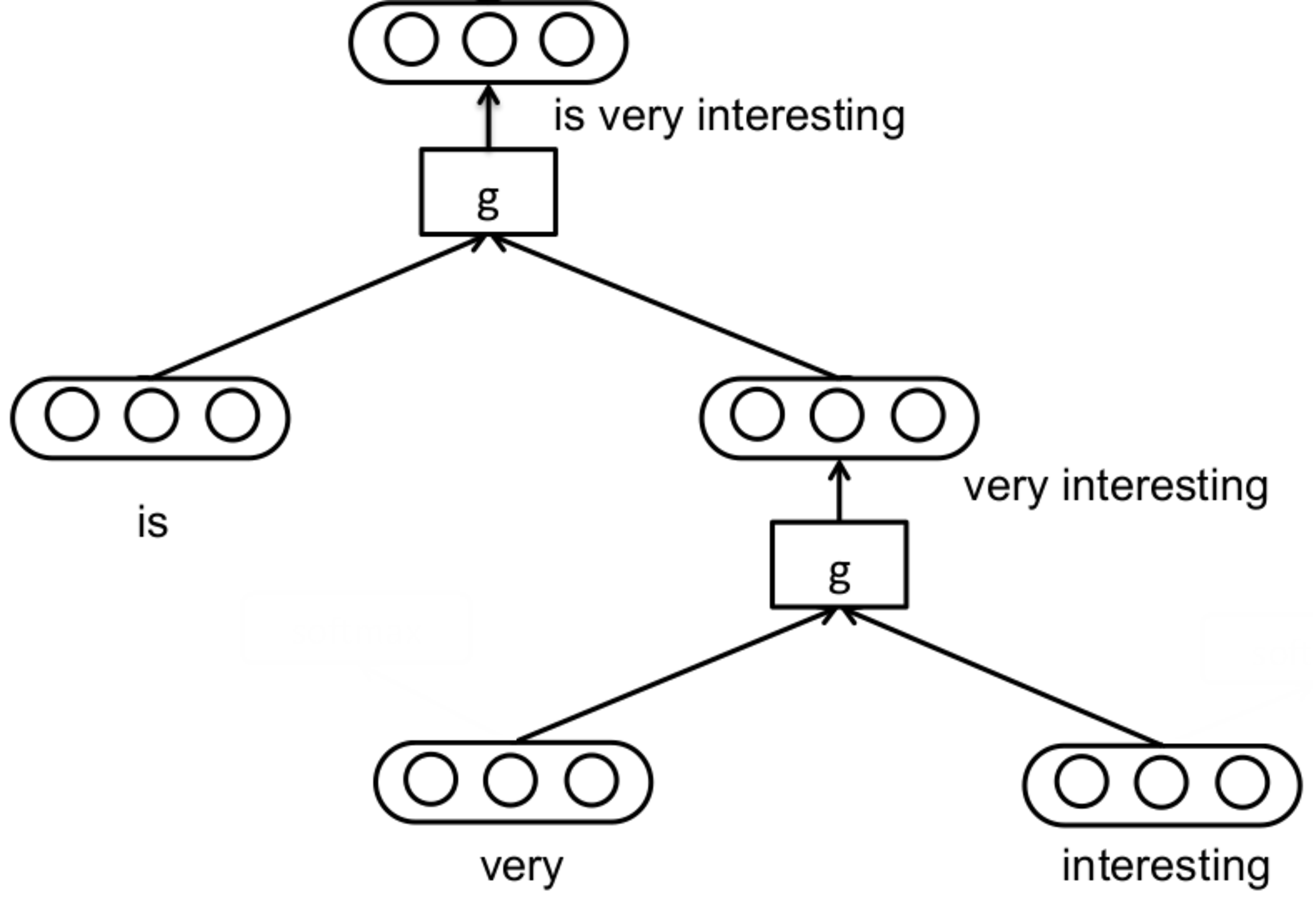
\includegraphics[scale=0.36]{figure/example-compose}
	\caption[Applying Recursive Neural Network on the phrase ``is very interesting'']{Applying Recursive Neural Network on the Constituency parse tree of the phrase ``is very interesting''.
		The composition function of this network is denoted as \textbf{g}.}
	\label{fig:example-compose}
\end{figure}

The core idea behind the design of Tree-LSTMs is to generalize the LSTMs for tree-structured inputs.
Tree-LSTMs were able to archive state-of-the-art performance on two tasks: predicting the semantic relatedness of two sentences (SemEval 2014, Task 1~\cite{SemeEvalTask1}) and sentiment classification (Stanford Sentiment Treebank~\cite{socher2013recursive}).

Let \(d\) be the size of the input vectors, \(r
\) be the size of the memory cell and \(z\) be the number of sentiment classes. 

\paragraph{Leaf module}
Given any input vector \(x \in \mathbb{R}^d\), the calculation steps inside the leaf module can be expressed as follow:
\begin{align}
o &= \sigma{\left( W^{(o)} x + a^{\left(o\right)}\right)} & \\
c &= W^{(c)} x + a^{(c)} & \\
h &= o \odot \tanh{\left(c\right)} &
\end{align}

In this module, \(W^{(o)}, W^{(c)} \in \mathbb{R}^{r \times d}\) and \(a^{\left(o\right)}, a^{(c)} \in \mathbb{R}^r\).

\paragraph{Composer module}
Given the input vectors \({h_l}\), \({c_l}\) from the left child node and \({h_r}\), \({c_r}\) from the right child node, the calculation steps inside the composer module can be expressed as follow:
\begin{align}
i &= \sigma{ \left(U_l^{(i)} h_{l} + U_r^{(i)} h_{r} + b^{(i)} \right) } &\\
f_{l} &= \sigma{\left(U_{l}^{(l)} h_{l} + U_{r}^{(l)} h_{r} + b^{(f)}\right)} & \\
f_{r} &= \sigma{\left(U_{l}^{(r)} h_{l} + U_{r}^{(r)} h_{r} + b^{(f)}\right)} & \\
o &= \sigma{\left( U_l^{(o)} h_{l} + U_r^{(o)} h_{r} + b^{(o)}\right)} &\\
u &= \tanh{\left( U_l^{(u)} h_{l} + U_r^{(u)} h_{r} + b^{(u)}\right)} &\\
c &= i \odot u + f_{l} \odot c_{l} + f_{r} \odot c_{r} & \\
h &= o \odot \tanh{\left(c\right)} &
\end{align}

In this module, for any \(j \in \{i, l, r, o, u\}\) and \(x \in \{\l, r\}\), \(U_x^{(j)} \in \mathbb{R}^{r \times r}\) and \( b^{(j)} \in \mathbb{R}^r\).

\paragraph{Composing sentence}
Given any sentence \({s}\) of length \({n}\) and its parse tree, originally, Tree-LSTM composes the output vectors by first applying its leaf module on each word vectors then applying its composition function at each node of the parse tree in a bottom-up manner.


\section{Challenges}
\subsection{Convolution and Pooling}
Although max-over-time pooling largely simplified the network (which is good for preventing over-fit), this solution have a clear drawback: the vector presentation of a sentence only tell if a feature appears in the sentence or not, the information about position of the feature is ignored.

\subsection{Recursive Neural Network}
\textbf{Tree-LSTMs also have some drawbacks}, these drawbacks including:
\begin{itemize}
	\item Sentences can be wrongly parsed, especially when comments are expressed in informal language.
	The performance of the system depends on the parser being used.
	\item At their leaf-module, Tree-LSTMs have only a simple logistic regression layer on top of the vector presentation of a single word at that position.
	The simple leaf-module of Tree-LSTMs might its weakness when dealing with the problem of words ambiguity.
	This weakness becomes even more severe when the sentence is wrongly parsed. 
\end{itemize}

\subsection{Word Embeddings}
There are many words (e.g. ``B-rated'', ``Batman'', ``Nolan'', ``cartoonlike'') which rarely appears in regular documents but more often in movie reviews.
Additionally, the ways people use words in movie reviews might be different from their usage in general documents.
For example, the vector presentations of ``sympathy'' and ``disappointed'', or ``boom'' and ``insult'' are very close to each other in Glove Common Crawl\footnote{Common Crawl (840B tokens, 2.2M vocab, cased, 300d vectors, 2.03 GB download) publicly available at \url{https://nlp.stanford.edu/projects/glove/}} but if we have to predict the sentiment of a movie comment which has one of these words, they should be distinctive.

Noticeably, many experiments~\cite{treeLSTM}~\cite{KimCNN} have shown that modifying word embeddings during the training process help improving performance of Deep Learning systems.
Although this method improves models' performance, it can harm generalization by updating only words which appear in the training set and not related words which only appear in test set.

\section{Method}
For dealing with the problem composing fixed size presentation vectors given variable-length input sentences, one intuitive solution would be to apply Recurrent Neural Networks~\cite{cnn-rnn}.
Another more complicated solution is utilizing Recursive Neural Networks.
\textbf{Recursive Neural Networks have several advantages over Recurrent Neural Networks}~\cite{need-tree}~\cite{bowman-treevslstm}: 
\begin{itemize}
	\item In case the input sequence belongs to recursively defined language, given only a small subset of the data with limited length sentences, tree structures model have better ability to generalize comparing to sequential ones.
	However, when we increase the limited length sentences, the advantage of tree over sequential models decrease fast~\cite{bowman-treevslstm}. 
	\item Tree can breaks down complicated sentences into simpler phrases, which make it easier for generalization~\cite{knowledge-matter}~\cite{need-tree}.
	\item Some features which are far apart when a sentence is presented as sequence become closer when it is presented as tree~\cite{need-tree}.
\end{itemize}

Different from Tree-LSTMs, CNN-multichannel's~\cite{KimCNN} first convolution layer have hundred of filters, each produces a feature map of the sentence by sliding through it with window sizes 3 to 5 words.
Filters with large context window help CNN-multichannel to mitigate the problem of words ambiguity and to capture phrase-level feature.
We think this is the reason why CNN-multichannel  can outperform TreeLSTMs, even when it have no respect for the positions of features. 

We combined Convolution Neural Networks with Tree-LSTM and sequential LSTM.
We hypothesized that the convolution layer will help Tree-LSTMs to mitigate the problem of lacking local context and words ambiguity at leaf nodes.
Additionally, using Tree-LSTM to combine the feature maps produced by the convolution layer might be a better choice compared to using max-over-time pooling layer.

We inserted a convolution layer between the word embedding layer and the Tree-LSTM's leaf-module.
The rest of TreeLSTM implementation was kept unchanged.
\subsection{Convolution Layer}
Given that \(F\) is the set of all filters of the convolution layer, for any filter \(v \in F\) which has window size \(l\) and set of parameters \(\theta^{(v)} = \{ W^{(v)}, b^{(v)} | W^{(v)} \in \mathbb{R}^{d \times l}, b^{(v)} \in \mathbb{R}\}\), filter \({v}\) is applied on any sequence of word-\(i\)th to word-\((i+l-1)\)th through the following equation:
\begin{align}
c^{(v)}_j &= f(W^{(v)} \otimes X_{i:i+l-1} + b^{(v)}) &\label{filter}
\end{align}

In Eq.\eqref{filter}, operator \(\otimes\) is the Hadamard product~\cite{element-prod}.  
\(b \in \mathbb{R}\) as bias term and \(f\) is an activation function.
For indexing, \(j = i + x\) with \(x \in \mathbb{N}\) and \(0 \leq x < l\).
If half-padding policy is employed then \(j = i + \floor{\frac{l}{2}}\).
For the case of multichannel input, given that the sentence is presented by any set of input channels \(Z\).
We will modify Eq.\eqref{filter} as follow:
\begin{align}
\forall h \in Z, \; \; \hat{c}^{(v)}_{jh} &= f(W^{(v)} \otimes X_{i:i+l-1} + b^{(v)})& \\
c^{(v)}_j &= \sum_{h \in Z} \hat{c}^{(v)}_{jh}&
\end{align}

By slicing the filter \(v\) through the sentence (i.e. applying the filter \(v\) on different sequences of length \(l\) along the sentence) we can get vector \(c^{(v)} = [c^{(v)}_0, c^{(v)}_1~\cdots]\) which is a feature map of the sentence \(s\).

Until now, we have not define the length of the feature map \(c^{(v)}\). 
To be able to work with Tree-LSTM (which required tree-structured inputs), all the feature maps produced by the convolution layer need to have length equal to that of the sentence \(s\) (which is \(n\) in this case).
For satisfying this constraint, all filters in \(F\) are restricted to have odd window sizes and being applied on the sentence according to half padding, unit strides policy~\cite{conv-arith}.
These conditions entail \({\forall u \in F,  c^{(u)} \in \mathbb{R}^n}\)~\cite{conv-arith}.


Suppose the size of set of filters \(F\) is \(m\), all the feature maps produced by the set of filters is then concatenated into one matrix \(P \in \mathbb{R}^{m \times n}\), which each of its row is a feature maps.
After that, the column vectors of \(P\) are treated as input vectors for Tree-LSTM or any Recurrent Neural Network.
\subsection{Recursive Neural Network}
For this module, we reused Constituency Tree-LSTM~\cite{treeLSTM}.


\subsubsection{Output Module and Loss Function}
 Denoting sequence of words spanned by a sub-tree rooted at node \({j}\) as \({\{x\}_j}\).
Given \({h_j}\) is the \({h}\) ouput of node \({j}\), the prediction at node \({j}\) can be computed by the output module as follow:
\begin{align}
\hat{p_{\theta}}(y \mid \{x\}_j ) &= softmax( W^{(s)} h_j + b^{(s)}) & \\
\hat{y_j} &= \underset{y}{\mathrm{argmax}} \; \hat{p_{\theta}}(y \mid \{x\}_j ) &
\end{align}

In this module, for any \(W^{(s)} \in \mathbb{R}^{z \times r}\) and \( b^{(s)} \in \mathbb{R}^z\).
For loss function, negative log-likelihood with \(L2\) regularization was used.

\subsubsection{Composing sentence}
In a case which convolution layer was added, the only difference is that for all \(0 \leq i \leq n-1\), the vector presentation of the word-\(i\)th is replaced with the \(i\)th-column of the matrix \(P\) produced by the convolution layer.
This mean the size of input vectors \(d\) is equal to the number of filters \(m\).

\subsection{Training Glove Vectors on Large Sentiment Dataset}
We observed that the available amount of document-level labeled sentiment data (e.g. Amazon Reviews dataset~\cite{amazon-reviews} has 83.68 million reviews) is gigantic compared to the amount of sentence or phrase-level sentiment data (e.g. Stanford Sentiment Treebank~\cite{socher2013recursive} has 8544 sentences in its training set, even it is the biggest sentence-level sentiment analysis dataset).
Although, there are some attempts to do transfer learning~\cite{group-instance}~\cite{re-embedding} (i.e. training on large document-level sentiment dataset then fine-tuning and/or test on sentence-level sentiment dataset), their performances are not high when evaluated on Stanford Sentiment Treebank~\cite{group-instance}.

We utilized Glove method to do transfer learning.
We hypothesized that by training Glove on review documents, especially movie or book reviews, we can capture more rare words and also the different way people use words (or different word relationships) to express their opinions on movies or books.
This might help our models archiving better generalisation when training on small sentence-level sentiment dataset like Stanford Sentiment Treebank~\cite{socher2013recursive}.

\section{Experiments}
\subsection{Datasets}
\subsubsection{Stanford Sentiment Treebank} \label{sec:sst}
In this thesis, we used Standford Sentiment Treebank (SST) dataset~\cite{socher2013recursive} to evaluate our models sentence-level sentiment analysis task.
Originally, the dataset was built based on Rotten Tomatoes Movie Review dataset~\cite{Rotten-Tomato}~\cite{socher2013recursive}.
In total, Standford Sentiment Treebank contains 11,855 sentences.
The dataset was split into training, validation and test set which contains 8544, 1101 and 2210 sentences respectively.


In this dataset, every sentence was parsed using Stanford (constituency) parser~\cite{socher2013recursive}\footnote{Open source tool: \url{https://stanfordnlp.github.io/CoreNLP/}}, each phrase which is spanned by any sub-tree of the parse tree is then labeled with  a fine-grained sentiment label.
Fine-grained sentiment is a setting which partition all sentiments into 5 classes: "Positive", "Somewhat Positive", "Neutral", "Somewhat Negative" and "Negative"~\cite{socher2013recursive} (a.k.a. \textbf{Fine-grained setting}).
There are total 215,154 phrases in the whole dataset.

For \textbf{Binary setting}, there are only to sentiment classed on the entire dataset, which means all neutral sentiment sentences are removed, "Positive" and "Somewhat Positive" are merged into one class, the same rule applied on "Somewhat Negative" and "Negative"~\cite{socher2013recursive}.
After all "Neutral" sentences have been removed, there are 6920/872/1821 sentences remained in train/dev/test set.

For training a Recurrent Neural Network on this dataset, any phrase which is spanned by a labeled node is treated as a training example. 

\subsubsection{Amazon Reviews}\label{sec:amazon}
Amazon Reviews is a gigantic review dataset
which contains 142.8 million reviews from Amazon spanning May 1996 - July 2014\footnote{\url{http://jmcauley.ucsd.edu/data/amazon/}}.
Each review contains product review (rating, text, helpfulness vote) and metadata (descriptions, category information, price, brand, and image features)~\cite{amazon-reviews}.
In this thesis, we only used a small part of Amazon Reviews.
These parts include Amazon Movies and TV reviews (7,850,072 reviews)~\cite{mcauley2013hidden}, Amazon Book reviews (22,507,155 reviews) and the new Movies and TV reviews (4,607,047 reviews)~\cite{McAuleyTSH15}~\cite{HeM16}.

\subsection{Experiment Setups}
We index all our experimented models along with their number of parameters in Table.\ref{table:paramtable}.

\begin{table}[H]
	\centering
	\caption{Number of trainable parameters of experimented models}
	\label{table:paramtable}
	\begin{tabular}{lll}
		~ & Memory Cell & Parameters count \\ \hline
		LSTM                     & 168         & 315,840          \\
		BiLSTM                   & 168         & 315,840          \\
		Constituency Tree-LSTM   & 150         & 316,800          \\
		Dependency Tree-LSTM     & 168         & 315.840          \\
		Constituency TE-Tree-GRU & 150         & 476,103          \\
		Dependency TE-Tree-GRU   & 150         & 316,353          \\
		CNN LSTM                 & 168         & 489,347          \\
		CNN Tree-LSTM            & 150         & 482,153          \\
		2 channel CNN LSTM       & 168         & 729,347          \\
		2 channel CNN Tree-LSTM  & 150         & 722,153
	\end{tabular}
\end{table}
\subsubsection{Hyper-parameters and Training}
For the models with only single input channel, we initialized word representation with Glove vectors~\cite{glove}.
With two word embeddings channels, we initialized one channel using Glove Common Crawl\footnote{\label{glovecommoncrawl}Common Crawl (840B tokens, 2.2M vocabularies, cased, 300d vectors, 2.03 GB download) publicly available at \url{https://nlp.stanford.edu/projects/glove/}} and the other using our Glove Amazon.

We tried a variety of convolution filters combination.
For single kernel size, we performed grid search on $\{100, 200, 300\}$ number of kernels of size $\{3, 5\}$.
For two different kernel size, we tried with $\{100, 200\}$ number of kernels for each kernel size.
Output matrices of different kernel sizes were concatenated as if they were with same kernel size.

Our model was trained using AdaGrad~\cite{duchi2011adaptive} with learning rate of $\{0.1,~ 0.05,~ 0.01\}$, L2 regularization of $\{1e^{-3},~ 1e^{-4}, ~ 1e^{-5} \}$, batch size of 25.
We manually update our word representation with learning rate $\alpha$ of $\{0.1,~0.05, ~0.01\}$ following Eq.\ref{eq:manuallyupdate}.
We regularized convolution layer with input dropout rate of 0.5 and output dropout rate of 0.2 in addition to dropout of rate 0.5 at output layer.
We applied the same hyper-parameters grid search for two channels convolution.
\begin{equation}
\label{eq:manuallyupdate}
w = w - \alpha\delta J(\theta)
\end{equation}

We found that 100 filters of size 3 words and 100 filters of size 5 words yield better results compared to single filters size or the number of filters larger than 200. We trained with Adagrad of learning rate of 0.01 and word vectors (updated manually) at learning rate 0.1 give the best result. We trained for 60 epochs for CNN Tree-LSTM and 20 epochs for CNN LSTM. Training 60 epochs on CNN LSTM did not yielded observable better result than 20 epochs.
\subsubsection{Glove Hyper-parameters and training}
Steps for preprocessing Amazon dataset for training word vectors on Glove:
\begin{enumerate}
	\item For retraining Glove vectors, we only used Amazon Movies and TV reviews dataset (7,850,072 reviews)~\cite{mcauley2013hidden}, Amazon Book reviews(22,507,155 reviews) and new Movies and TV dataset (4,607,047 reviews)~\cite{McAuleyTSH15}~\cite{HeM16}.
	\item All the reviews were grouped by product-ID ("asin" keyword in the JSON schema of the dataset).
	\item In each product-ID group, the reviews were sorted increasingly by their rating ("overall" keyword in the JSON schema of the dataset).
	\item All the reviews were dumped into a plain text file.
	\item The text file produced from the previous step was tokenized using Stanford Tokenizer~\cite{tokenizerpart}.
\end{enumerate}

The reason for doing step 2 and step 3 is because there is no definition of end-of-document in Glove model, which means words which appear in the beginning part of a document will be included in the context of words in the last part of the previous document which leads to noise in training data. Step 2 and 3 help us to mitigate this problem.

We use Glove implementation\footnote{Publicly available on Github \url{https://github.com/stanfordnlp/GloVe}} to train word representation.
We set $x_{max} = 100$, vector size to 300, windows size to 20 and the minimum number of word occurrences to be included in the vocabulary to 5.
The training process took the plain text file produced by the preprocessing steps as its input.
In total, the size of the corpus is 4.7 billions tokens.
After the training process, the resulting word embeddings has vocabulary size of 1,734,244.
We named this word embeddings Glove Amazon.

For evaluating, we used Glove Amazon to replace Glove Common Crawl for initializing word embedding layer of Tree-LSTM.
Apart from that, the whole training process and hyper-parameters are kept unchanged.

\subsection{Results and Discussion}

\begin{table*}[]
	\centering
	\caption[Experiment result on SST]{Experiment results of models evaluated on Stanford Sentiment Treebank with binary setting.
		The models which have both data of mean(std) and max are models which have been evaluated by us.
		For these models, we report mean, standard deviation and max of 5 runs.
		If a model has data of only mean(std) or only max, the data was taken from its originated research paper.
		If the data of both mean(std) and max is missing, the model was not evaluated yet.
		\textit{(*): Result reported by the original paper.}}
	\label{table:experimentresult}
	\begin{tabular}{c|lll}
		\textbf{Block}    & \textbf{Model}  & \textbf{Mean(std)} & \textbf{Max}   \\
		\Xhline{3\arrayrulewidth}
		\Xhline{3\arrayrulewidth}
		
		\multirow{4}{*}{A} & CNN-non-static~\cite{KimCNN} & - & 87.20\Tstrut \\
		& CNN-multichannel~\cite{KimCNN} & - & 88.10 \\
		& DCNN~\cite{DCNN} & - & 86.80 \\
		& MVCNN~\cite{2-layer-cnn} & - & 89.40 \\
		\hline
		\multirow{5}{*}{B} & LSTM~\cite{originLSTM}    & 86.64 (0.27) & 86.93  \\
		& BiLSTM~\cite{GravesLSTM}  & 85.80 (0.69) & 86.43   \\
		& 2-layer LSTM~\cite{GravesLSTM} & 86.30 (0.60) & - \\
		& 2-layer Bidirectional LSTM~\cite{GravesLSTM} & 87.20 (1.00) & - \\
		& DMN~\cite{attention-gru} & - & 88.60 \\
		\hline
		\multirow{5}{*}{C} & RNTN~\cite{socher2013recursive}  & - & 85.40  \\
		& DRNN~\cite{IrsoyDRNN} & - & 86.60 \\
		& TE-RNTN~\cite{tag-embedding-rnn} & - & 87.70 \\
		& Dependency Tree-LSTM  ~\cite{treeLSTM}  & 85.70 (0.30)  & 85.80 \\
		& Constituency Tree-LSTM ~\cite{treeLSTM} & 88.00 (0.40)    &   88.19\\
		\hline
		\multirow{2}{*}{E}  & CNN GRU ~\cite{cnn-rnn}                    & 89.13 (0.29)  &  89.61 (89.95)*    \\
		& CNN LSTM ~\cite{cnn-rnn}                    & 89.43 (0.28)  & 89.72 (89.56)*\Bstrut    \\
		\Xhline{3\arrayrulewidth}
		\Xhline{3\arrayrulewidth}
		 & Constituency Tree-LSTM ~\cite{treeLSTM} (Glove Amazon) & 88.85 (0.44) & 89.35\Tstrut\\
		& 2 Channel CNN LSTM                        & 89.54    (0.22) & 89.79    \\
		 & CNN Tree-LSTM                            & 88.82 (0.13) & 88.92 \\
		& CNN Tree-LSTM (Glove Amazon)             & 88.96 (0.24) & 89.18 \\
		& 2 Channel CNN Tree-LSTM  &\textbf{89.69 (0.36)} & \textbf{90.12}    \\
	\end{tabular}
\end{table*}


% \textit{(***): CNN and LSTM layer are initialize using pre-trained parameters from Section \ref{sec:CNNtree}}

Experiment results are summaries in Table \ref{table:experimentresult}.
Table \ref{table:experimentresult} is divided into two parts.
The first part is from Block A to E, which contains all baselines model.
The second part is from Block F to I, which contains all models which were proposed and evaluated by us.

\textbf{Descriptions of each Block in the first part}:
\begin{description}
	\item[Block A] contains Multilayer Convolution Neural Networks models.
	CNN-non-static and CNN-multichannel~\cite{KimCNN} are single layer CNN.
	DCNN~\cite{DCNN} and MVCNN~\cite{2-layer-cnn} are multilayer CNN, with MVCNN is a very large model  which has 2 layers, 5 word embeddings channels and unsupervised pre-train using the method of Sentence Encoding.
	\item[Block B] contains sequential/recurrent models.
	LSTM~\cite{originLSTM}, BiLSTM~\cite{GravesLSTM}, 2-layer LSTM~\cite{GravesLSTM} and 2-layer Bidirectional LSTM~\cite{GravesLSTM} have been described in Sec??.\ref{sec:RNN}.
	DMN~\cite{attention-gru} is a sophisticated model used GRU with attention mechanism and episodic memory.
	\item[Block C] contains models which belong to the family of Recursive Neural Networks (tree-structured model).
	RNTN~\cite{socher2013recursive} is the first recursive neural network to successfully apply on sentence-level sentiment analysis (Stanford Sentiment Treebank).
	It was inspired by the idea that natural languages have recursive structure, to understand a sentence we must understand its phrases and, to understand a phrase, we must understand its words.
	DRNN~\cite{IrsoyDRNN} is a multilayered extension of RNTN.
	TE-RNTN is also an extension of RNTN which utilize the local syntactic information at each node of a sentence's parse tree.
	Dependency and Constituency Tree-LSTM~\cite{treeLSTM} are tree-structured versions of LSTM.
	
	\item[Block E] contains models which combine Convolution Neural Networks and Recurrent Neural Networks.
	CNN GRU and CNN LSTM~\cite{cnn-rnn} have been described in detail in Sec.\ref{cnn-rnn}.
	In our experiments with CNN GRU and CNN LSTM, we used the implementation publicly published by the authors\footnote{\url{https://github.com/ultimate010/crnn}}.
\end{description}
\subsubsection{Transfer Learning by retraining Glove on Amazon Reviews dataset}
\label{fact:glove-amazon-improve-tree}
In Block G, Constituency Tree-LSTM using Glove Amazon largely outperformed Constituency Tree-LSTM using Glove Common Crawl even though it was trained on significantly larger dataset (840B tokens) compared to our preprocessed Amazon Reviews (4.7B tokens).

Compared to Glove Amazon method, originally,  Paragraph-Vec~\cite{ParagraphVec} cannot be fine-tuning in a supervised manner.
We also used PARAGRAM-SL999 for initializing the word embeddings layer of Constituency Tree-LSTM,
the results (of 8 runs with mean 87.175\% and standard deviation 0.69) were not as good as those of Glove Common Crawl.

These results support our hypothesis that by training word embeddings on review documents, especially movie or book reviews, we can capture more rare words and also the different way people use words (or different word relationships) when they express their opinions on movies or books.

\subsubsection{Combining Recursive Neural Networks with Convolution Neural Networks}
\label{proved:tree-conv-benefit}
The fact that CNN Tree-LSTM outperforms Constituency Tree-LSTM~\cite{treeLSTM} supports our hypothesis on the benefits of combining convolution layers with Tree-LSTM.
Due to using similar architects, CNN LSTM was comparable with CNN GRU and CNN LSTM~\cite{cnn-rnn}. \label{unproved:cnn-treelstm-overfit}
CNN Tree-LSTM performed worst than CNN LSTM, the reason might because of over-fitting.
We will prove this hypothesis by looking at the plots of error rate on training and validation set of these two models.

\label{proved:Amazon-adv-Common}
We have seen that Glove Amazon improved Tree-LSTM in Sec.\ref{fact:glove-amazon-improve-tree}.
In these experiments (Block I), Glove Amazon also improved CNN Tree-LSTM.
We can conclude that Amazon Glove captured some good\footnote{good for the task of sentiment analysis of movie reviews} features that does not exist or hardly be extracted in Glove Common Crawl.

According to Table.\ref{table:paramtable}, the number of parameters of 2 Channel CNN Tree-LSTM (722,153) is much larger than that of CNN Tree-LSTM (482,153), which makes it more likely for 2 Channel CNN Tree-LSTM to over-fit the training data.
However, in fact, 2 Channel CNN Tree-LSTM was able to archive much higher accuracy than both CNN Tree-LSTM (Glove Amazon) and CNN Tree-LSTM (Glove Common Crawl).\label{proved:Common-syn-Amazon}
The result proves that there are some features only appearing in Glove Common Crawl or when combining both Glove Amazon and Glove Common Crawl.
Otherwise, there would not be any improvement.

\section{Conclusion}
\subsection{Future works}
In many cases, the sentiment class of a sentence can only be revealed through multiple steps of induction and deduction on a knowledge base.
We suspected that most of the networks we have done experiments with (e.g. Tree-LSTMs, CNN-multichannel and our model) do the sentiment classification task based on detecting features and do not rely on induction or deduction.
We thinks that most of the knowledge these models have is embedded in their word embeddings (which have 6,255,600 parameters or double that number in case of two input channels compared to 722,153 parameters at most in these neural networks).

In recent years, Recurrent Neural Networks with external memory~\cite{Graves_Nature2016}~\cite{neural-turing-machine} have come into sight.
DNC~\cite{Graves_Nature2016} was proved to have certain level of reasoning on the bAbI dataset~\cite{bAbi}.
We hope that we can apply this reasoning ability on sentence-level sentiment analysis.

\appendix
%Appendix A

\begin{acks}
  The authors would like to thank Dr. Yuhua Li for providing the
  matlab code of  the \textit{BEPS} method. 

  The authors would also like to thank the anonymous referees for
  their valuable comments and helpful suggestions. The work is
  supported by the \grantsponsor{GS501100001809}{National Natural
    Science Foundation of
    China}{http://dx.doi.org/10.13039/501100001809} under Grant
  No.:~\grantnum{GS501100001809}{61273304}
  and~\grantnum[http://www.nnsf.cn/youngscientsts]{GS501100001809}{Young
    Scientsts' Support Program}.

\end{acks}


\bibliographystyle{ACM-Reference-Format}
\bibliography{sample-bibliography} 

\end{document}
